% Options for packages loaded elsewhere
\PassOptionsToPackage{unicode}{hyperref}
\PassOptionsToPackage{hyphens}{url}
%
\documentclass[
  ignorenonframetext,
]{beamer}
\usepackage{pgfpages}
\setbeamertemplate{caption}[numbered]
\setbeamertemplate{caption label separator}{: }
\setbeamercolor{caption name}{fg=normal text.fg}
\beamertemplatenavigationsymbolsempty
% Prevent slide breaks in the middle of a paragraph
\widowpenalties 1 10000
\raggedbottom
\setbeamertemplate{part page}{
  \centering
  \begin{beamercolorbox}[sep=16pt,center]{part title}
    \usebeamerfont{part title}\insertpart\par
  \end{beamercolorbox}
}
\setbeamertemplate{section page}{
  \centering
  \begin{beamercolorbox}[sep=12pt,center]{part title}
    \usebeamerfont{section title}\insertsection\par
  \end{beamercolorbox}
}
\setbeamertemplate{subsection page}{
  \centering
  \begin{beamercolorbox}[sep=8pt,center]{part title}
    \usebeamerfont{subsection title}\insertsubsection\par
  \end{beamercolorbox}
}
\AtBeginPart{
  \frame{\partpage}
}
\AtBeginSection{
  \ifbibliography
  \else
    \frame{\sectionpage}
  \fi
}
\AtBeginSubsection{
  \frame{\subsectionpage}
}
\usepackage{lmodern}
\usepackage{amssymb,amsmath}
\usepackage{ifxetex,ifluatex}
\ifnum 0\ifxetex 1\fi\ifluatex 1\fi=0 % if pdftex
  \usepackage[T1]{fontenc}
  \usepackage[utf8]{inputenc}
  \usepackage{textcomp} % provide euro and other symbols
\else % if luatex or xetex
  \usepackage{unicode-math}
  \defaultfontfeatures{Scale=MatchLowercase}
  \defaultfontfeatures[\rmfamily]{Ligatures=TeX,Scale=1}
\fi
\usecolortheme{beaver}
\usefonttheme{structurebold}
% Use upquote if available, for straight quotes in verbatim environments
\IfFileExists{upquote.sty}{\usepackage{upquote}}{}
\IfFileExists{microtype.sty}{% use microtype if available
  \usepackage[]{microtype}
  \UseMicrotypeSet[protrusion]{basicmath} % disable protrusion for tt fonts
}{}
\makeatletter
\@ifundefined{KOMAClassName}{% if non-KOMA class
  \IfFileExists{parskip.sty}{%
    \usepackage{parskip}
  }{% else
    \setlength{\parindent}{0pt}
    \setlength{\parskip}{6pt plus 2pt minus 1pt}}
}{% if KOMA class
  \KOMAoptions{parskip=half}}
\makeatother
\usepackage{xcolor}
\IfFileExists{xurl.sty}{\usepackage{xurl}}{} % add URL line breaks if available
\IfFileExists{bookmark.sty}{\usepackage{bookmark}}{\usepackage{hyperref}}
\hypersetup{
  pdftitle={Analyzing the influence of Selection on Genetic Programming's Generalization ability in Symbolic Regression},
  hidelinks,
  pdfcreator={LaTeX via pandoc}}
\urlstyle{same} % disable monospaced font for URLs
\newif\ifbibliography
\usepackage{graphicx}
\makeatletter
\def\maxwidth{\ifdim\Gin@nat@width>\linewidth\linewidth\else\Gin@nat@width\fi}
\def\maxheight{\ifdim\Gin@nat@height>\textheight\textheight\else\Gin@nat@height\fi}
\makeatother
% Scale images if necessary, so that they will not overflow the page
% margins by default, and it is still possible to overwrite the defaults
% using explicit options in \includegraphics[width, height, ...]{}
\setkeys{Gin}{width=\maxwidth,height=\maxheight,keepaspectratio}
% Set default figure placement to htbp
\makeatletter
\def\fps@figure{htbp}
\makeatother
\setlength{\emergencystretch}{3em} % prevent overfull lines
\providecommand{\tightlist}{%
  \setlength{\itemsep}{0pt}\setlength{\parskip}{0pt}}
\setcounter{secnumdepth}{5}

\title{Analyzing the influence of Selection on Genetic Programming's
Generalization ability in Symbolic Regression}
\subtitle{A comparison of epsilon-lexicase Selection and Tournament
Selection}
\author{}
\date{\vspace{-2.5em}2022-06-29}

\begin{document}
\frame{\titlepage}

\begin{frame}[allowframebreaks]
  \tableofcontents[hideallsubsections]
\end{frame}
\hypertarget{introduction}{%
\section{Introduction}\label{introduction}}

\begin{frame}{Research Question}
\protect\hypertarget{research-question}{}
\begin{itemize}
\tightlist
\item
  Does the usage of \(\epsilon\)-lexicase parent selection influence the
  generalization behaviour of genetic programming in symbolic regression
  if compared to tournament selection?
\end{itemize}
\end{frame}

\begin{frame}{Genetic Programming}
\protect\hypertarget{genetic-programming}{}
\begin{itemize}
\tightlist
\item
  A metaheuristic that searches for computer programs that solve a given
  problem
\item
  Evolutionary algorithm that simulates the process of Darwinian
  evolution:

  \begin{enumerate}
  \tightlist
  \item
    Fitnessfunction: Evaluates the quality of a solution
  \item
    Selection: Solutions are selected based on their individual fitness
  \item
    Variation: Mutation and recombination of solutions
  \end{enumerate}
\item
  Unique Features:

  \begin{itemize}
  \tightlist
  \item
    Evolve solutions of variable length and structure
  \item
    Solutions are typically represented by recursive tree structures
  \end{itemize}
\end{itemize}
\end{frame}

\begin{frame}{Parent Selection}
\protect\hypertarget{parent-selection}{}
\ldots{}
\end{frame}

\begin{frame}{Symbolic Regression}
\protect\hypertarget{symbolic-regression}{}
\ldots{}
\end{frame}

\begin{frame}{Generalization}
\protect\hypertarget{generalization}{}
\end{frame}

\begin{frame}{Motivation}
\protect\hypertarget{motivation}{}
\begin{itemize}
\tightlist
\item
  Generalization
\end{itemize}
\end{frame}

\hypertarget{theoretical-foundations}{%
\section{Theoretical Foundations}\label{theoretical-foundations}}

\begin{frame}{Genetic Programming}
\protect\hypertarget{genetic-programming-1}{}
\ldots{}

\ldots{}
\end{frame}

\hypertarget{experimental-study}{%
\section{Experimental Study}\label{experimental-study}}

\begin{frame}{Experimental Study}
\ldots{}
\end{frame}

\begin{frame}{Research Design}
\protect\hypertarget{research-design}{}
\ldots{}
\end{frame}

\begin{frame}{Genetic Programming Configuration}
\protect\hypertarget{genetic-programming-configuration}{}
\ldots{}
\end{frame}

\hypertarget{results}{%
\section{Results}\label{results}}

\begin{frame}{Descriptive Statistics}
\protect\hypertarget{descriptive-statistics}{}
\begin{figure}
\centering
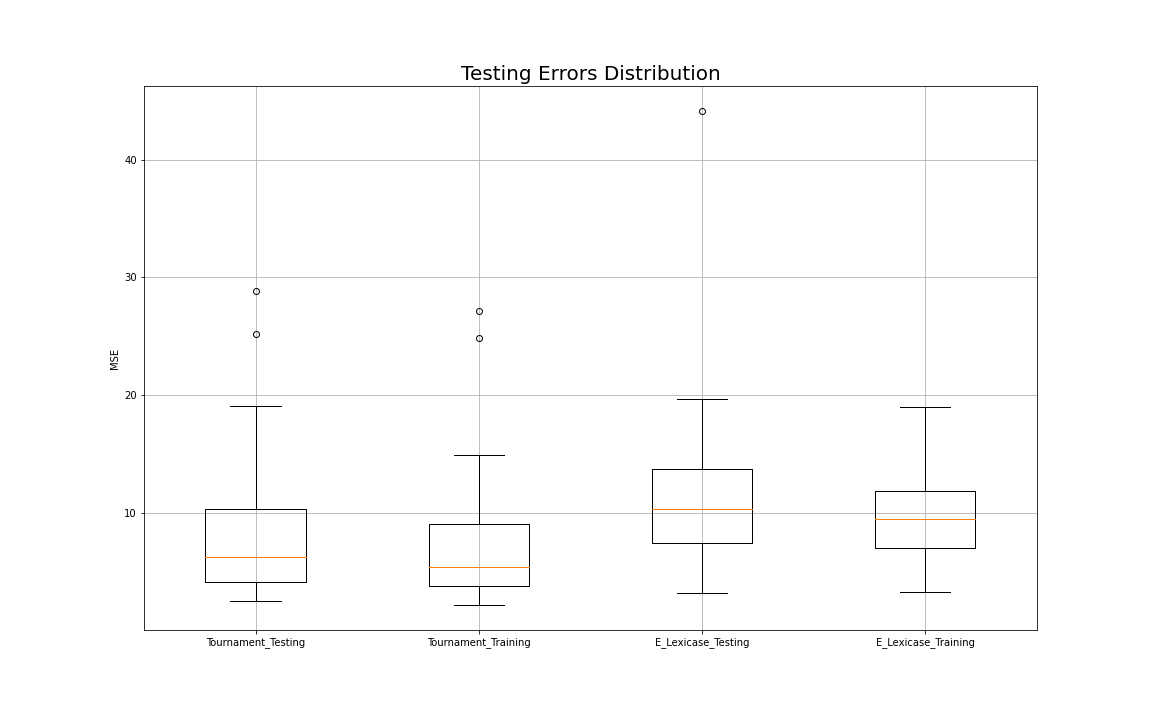
\includegraphics{../plots/mean_error_boxplot_all.png}
\caption{Distribution of Errors}
\end{figure}

\ldots{}
\end{frame}

\hypertarget{conclusions}{%
\section{Conclusions}\label{conclusions}}

\begin{frame}{Conclusions}
\ldots{}
\end{frame}

\hypertarget{limitations-and-open-questions}{%
\section{Limitations and open
Questions}\label{limitations-and-open-questions}}

\begin{frame}{Limitations and open Questions}
\ldots{}
\end{frame}

\hypertarget{references}{%
\section{References}\label{references}}

\end{document}
